%\documentstyle[epsf,twocolumn]{jarticle}       %LaTeX2.09仕様
%\documentclass[twocolumn]{jarticle}     %pLaTeX2e仕様
\documentclass[twocolumn]{jarticle}     %pLaTeX2e仕様

\setlength{\topmargin}{-45pt}
%\setlength{\oddsidemargin}{0cm} 
\setlength{\oddsidemargin}{-7.5mm}
%\setlength{\evensidemargin}{0cm} 
\setlength{\textheight}{24.1cm}
%setlength{\textheight}{25cm} 
\setlength{\textwidth}{17.4cm}
%\setlength{\textwidth}{172mm} 
\setlength{\columnsep}{11mm}

\kanjiskip=.07zw plus.5pt minus.5pt

\usepackage{graphicx}
\usepackage[dvipdfmx]{color}
\usepackage{subcaption}
\usepackage{enumerate}
\usepackage{comment}
\usepackage{url}
\usepackage{multirow}
\usepackage{diagbox}
\usepackage{bm}



\begin{document}
\twocolumn[
  \noindent
  \hspace{1em}

  \today
  \hfill
  \ \  学籍番号1201201100 西村昭賢 

  \vspace{2mm}
  \hrule
  \begin{center}
  {\Large \bf 情報工学英語演習 「{\rm AttentionIsAllYouNeed}」の和訳}
  \end{center}
  \hrule
  \vspace{3mm}
]

\section*{Abstruct}
今までの主要なsequence transduction modelは,エンコーダーとデコーダーを含む
複雑なRNNやCNNに基づいていた.最も良いパフォーマンスであったモデルも,エンコーダーとデコーダーをアテンションの仕組みを用いて接続しているモデルであった.\par
私達は,RNNやCNNを用いず,アテンションのみからなるTransformerと呼ばれる新しい簡潔なモデルを提案する.2回の翻訳実験の結果,Transformerは今までのモデルより優れており,更には,より並列化が可能で学習の時間も少ないことが分かった.
TransformerはWMT2014英独翻訳タスクにおいて,「プロの翻訳者の訳と近ければ近いほどその機械翻訳の精度は高い」という考え方に基づく機械翻訳の評価方法であるBLEUスコアで28.4BLEUを記録した.これは,複数のモデルを融合させて1つの学習モデルを生成するアンサンブル学習を含めたこれまでの最高記録を2BLEU上回る結果であった.また、WMT2014英仏翻訳タスクにおいては、8個のGPUを用いた3.5日の学習というこれまでの最先端のモデルの学習よりも遥かに少ないコストで,41.0BLEUという単一モデルの最高記録を打ち立てた.

%TODO sequence transduction modelの自然な訳、時系列分析モデル?


\section{Introduction}
RNN,特にRNNにおいて文章の長期的な依存関係を学習できるようにしたLSTMやgated RNNは,言語モデルや機械翻訳などのSequence 問題への最適な手法として確固たる地位を築いていた.
それ以来,Recurrent言語モデルとエンコーダー-デコーダー構造の限界を押し上げる数々の努力がなされてきた.
\par
リカレントモデルでは,通常,入力と出力の時系列データの時間的な位置に沿って計算を行う.
よって計算は逐次的に行われ,時刻$t$における隠れ状態$h_\mathrm{t}$は,時刻$t-1$の隠れ状態の$h_\mathrm{t-1}$と時刻$t$における入力から導かれる.
このように本質的に逐次的な性質を孕んでいるため,学習の並列処理が困難である.そのため,メモリの制約上,長い時系列データなどの学習には致命的であった.
直近の研究ではfactorization tricksやconditional computationといった方法で計算効率がかなり改善され,後者ではモデルの性能まで向上させることができたが,逐次的な計算の問題は残ったままだった.\par
Attentionは入力と出力の時系列データにおける距離を気にせず依存関係をモデル化することができ,様々なタスクにおいて有効なsequence modelとtransduction modelの必要不可欠な部分となっている.しかし,一部の場合にはAttentionはRNNと合わせて用いられる.\par
本研究で私達が提案するTransformerは,RNNを用いず,Attentionのみで入力と出力の完全な依存関係を取り出すモデルのアーキテクチャである.
Transformerは学習の並列処理が可能であり,8個のP100 GPUで12時間という小規模な学習後に,最高の機械翻訳性能に達することができた.


\section{BackGround}
逐次的な計算を減らすという目標は,Extended Neural GPU,ByteNet,ConvS2Sといったモデルの基礎にもなっている.これらはどれもCNNを基本構成要素として,入力と出力のすべての位置で隠れ状態の値を計算する.またこれらのモデルにおいて,任意の入力の位置と出力の位置の信号を関連付けるために必要な計算時間は,ConvS2Sdでは線形的,ByteNetでは指数的となる.
そのため離れた位置の依存関係を学習することはより困難になる.
Transformerでは,この計算時間を定数時間に減らすことができる.Attentionで重み付けした位置を平均化することで有効な解像度が下がってしまうが,3.2説で述べるMulti-Head Attentionにより相殺できる.\par

intra-attentionとも呼ばれるSelf-Attentionは,単一の文章の異なる位置を関連付けるAttentionである.Self-Attentionは文章読解,要約,テキスト含意,独立した文の表現の学習などのタスクで用いられ成功している.\par

End-to-End memory NetworksはRNNの代わりに再帰的なAttentionを元にしており,単純な言語の質疑応答,言語モデリングといったタスクにおいて優れた結果を示している.\par

しかし私達が知る限り,TransformerはRNNやCNNを用いずに入出力の表現を計算するために,Self-Attentionのみに依存した最初のtransduction modelである.次節以降では,Transformer,self-attentionについて説明しこれまでのモデルと比較した利点を議論する.




\section{Model Architecture}
最も優位性のあるsequence transduction modelsはエンコーダー-デコーダー構造を有している.エンコーダーは配列で表現される入力($x_\mathrm{1}$,...,$x_\mathrm{n}$)を配列\bm{$z$}=($z_\mathrm{1}$,...,$z_\mathrm{n}$)に変換する.
デコーダーは\bm{$z$}から出力として配列($y_\mathrm{1}$,...,$y_\mathrm{n}$)を1要素ずつ出力する.
このステップで,モデルが生成する要素はこれまでに生成した要素のみに依存する自己回帰モデルであり,直前に生成された要素を新しく入力として次の要素を生成する.\par
Transformerは図1の左半分と右半分に示すように,全体としてはエンコーダー-デコーダー構造を踏襲しつつ,self-attention層とpoint-wise全結合層を積み重ねた層を使用している.

\begin{figure}[ht]
  \centering
  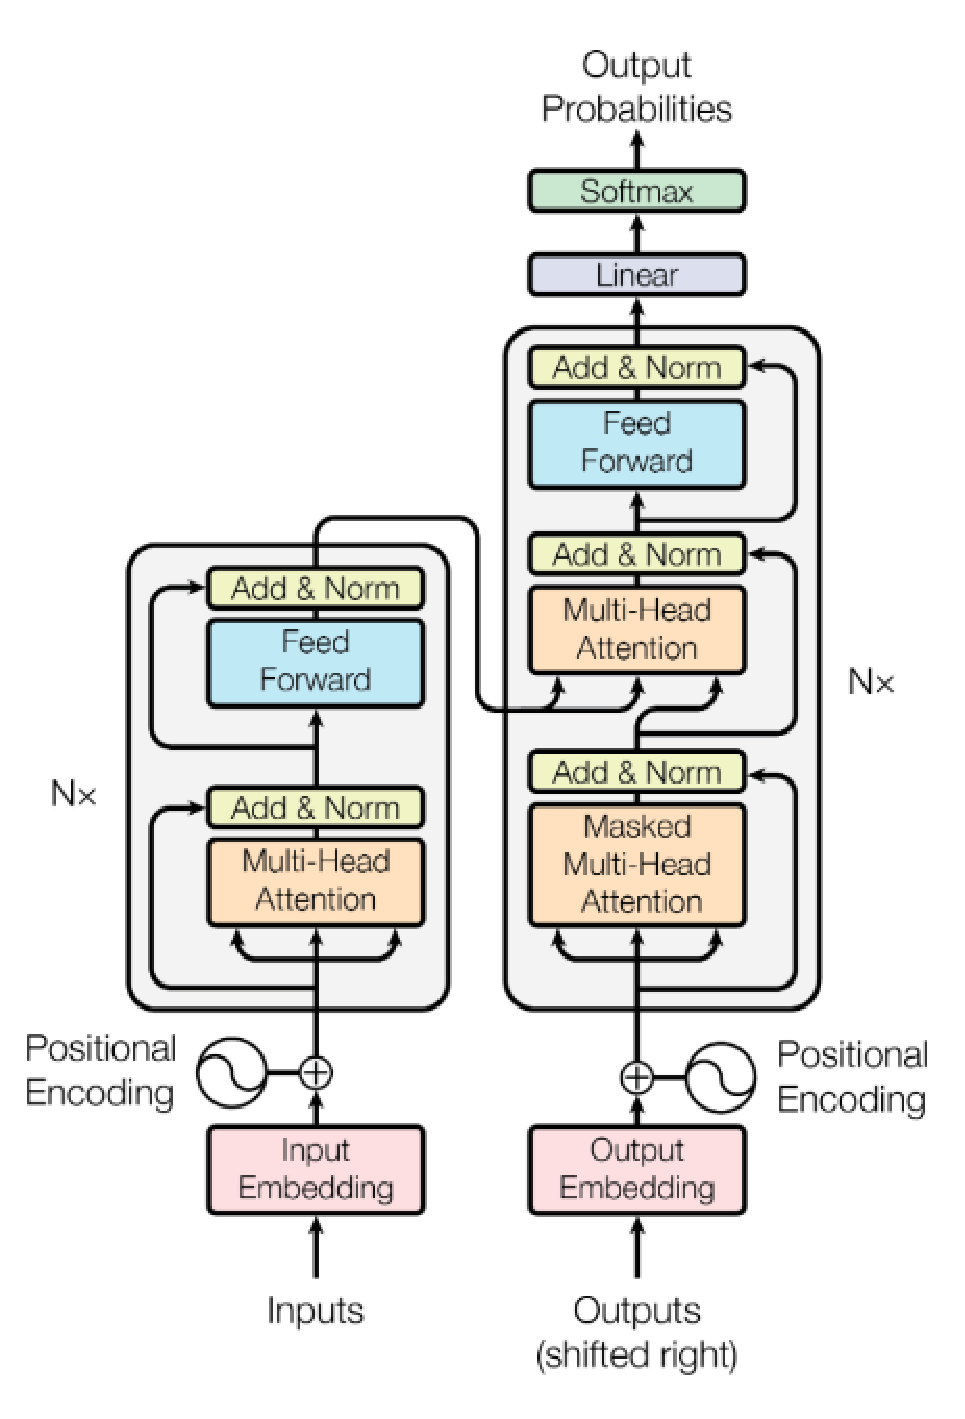
\includegraphics[width=75mm]{assets/Figure1.eps}
  \caption{図1: Transformerのモデルアーキテクチャ}
  \label{fig:vote_Accuracy}
\end{figure}


\subsection{Encoder and Decoder Stacks}
???
\subsection{Attention}

\subsubsection{Scaled Dot-Product Attention}

\subsubsection{Multi-Head Attention}

\subsubsection{Applications of Attention in our Model}

\subsection{Position-wise Feed-Forward Networks}

\subsection{Embeddings and Softmax}

\subsection{Positional Encoding}

\section{Why Self-Attention}

\section{Training}

\subsection{Training Data and Batching}

\subsection{Hardware and Schedule}

\subsection{Optimizer}

\subsection{Regularization}

\section{Results}

\subsection{Machine Translation}

\subsection{Model Variations}

\section{Conclusion}

%TODO 用語説明的な部分の書き方調べる

%index.bibはtexファイルと同階層に置く
%ちゃんと\citeしないと表示されない(1敗)
\bibliography{index.bib}
\bibliographystyle{junsrt}

\end{document}